\begin{figure}[H]
\centering
\begingroup\color{black}
\definecolor{personBlue}{RGB}{0,92,166}\definecolor{personOrange}{RGB}{217,91,0}
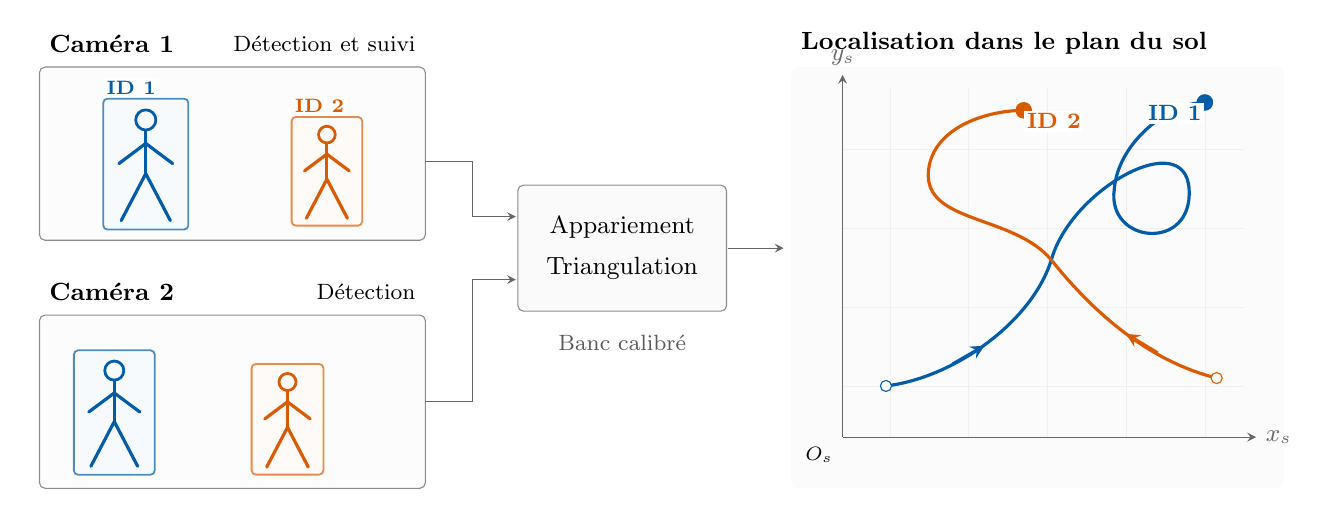
\begin{tikzpicture}[x=1cm,y=1cm,font=\small,>=stealth]
\path[use as bounding box] (-.15,.5) rectangle (15.9,6.5);
\node[anchor=west,font=\bfseries\small] at (0,6.3) {Caméra 1};
\node[anchor=east,font=\footnotesize] at (4.9,6.3) {Détection et suivi};
\draw[black!45,rounded corners=2pt,fill=gray!2] (0,3.8) rectangle (4.9,6.0);
\node[anchor=west,font=\bfseries\small] at (0,3.15) {Caméra 2};
\node[anchor=east,font=\footnotesize] at (4.9,3.15) {Détection};
\draw[black!45,rounded corners=2pt,fill=gray!2] (0,.65) rectangle (4.9,2.85);

\draw[personBlue!70,line width=.65pt,rounded corners=1.5pt,fill=personBlue!3] (0.810,3.936) rectangle (1.890,5.598);
\draw[personBlue,line width=1pt,line cap=round,line join=round] (1.350,5.328) circle (0.128);
\draw[personBlue,line width=1.15pt,line cap=round,line join=round] (1.350,5.186)--(1.350,4.646);
\draw[personBlue,line width=1.15pt,line cap=round,line join=round] (1.009,4.774)--(1.350,5.030)--(1.691,4.774);
\draw[personBlue,line width=1.15pt,line cap=round,line join=round] (1.038,4.050)--(1.350,4.646)--(1.662,4.050);
\node[anchor=south west,font=\scriptsize\bfseries,text=personBlue,fill=white,inner sep=1pt] at (0.810,5.612) {ID 1};
\draw[personOrange!70,line width=.65pt,rounded corners=1.5pt,fill=personOrange!3] (3.202,3.986) rectangle (4.098,5.366);
\draw[personOrange,line width=1pt,line cap=round,line join=round] (3.650,5.142) circle (0.106);
\draw[personOrange,line width=1.15pt,line cap=round,line join=round] (3.650,5.024)--(3.650,4.576);
\draw[personOrange,line width=1.15pt,line cap=round,line join=round] (3.367,4.682)--(3.650,4.894)--(3.933,4.682);
\draw[personOrange,line width=1.15pt,line cap=round,line join=round] (3.390,4.080)--(3.650,4.576)--(3.910,4.080);
\node[anchor=south west,font=\scriptsize\bfseries,text=personOrange,fill=white,inner sep=1pt] at (3.202,5.378) {ID 2};
\draw[personBlue!70,line width=.65pt,rounded corners=1.5pt,fill=personBlue!3] (0.437,0.822) rectangle (1.463,2.402);
\draw[personBlue,line width=1pt,line cap=round,line join=round] (0.950,2.145) circle (0.121);
\draw[personBlue,line width=1.15pt,line cap=round,line join=round] (0.950,2.010)--(0.950,1.497);
\draw[personBlue,line width=1.15pt,line cap=round,line join=round] (0.626,1.619)--(0.950,1.861)--(1.274,1.619);
\draw[personBlue,line width=1.15pt,line cap=round,line join=round] (0.653,0.930)--(0.950,1.497)--(1.247,0.930);
\draw[personOrange!70,line width=.65pt,rounded corners=1.5pt,fill=personOrange!3] (2.694,0.824) rectangle (3.606,2.228);
\draw[personOrange,line width=1pt,line cap=round,line join=round] (3.150,2.000) circle (0.108);
\draw[personOrange,line width=1.15pt,line cap=round,line join=round] (3.150,1.880)--(3.150,1.424);
\draw[personOrange,line width=1.15pt,line cap=round,line join=round] (2.862,1.532)--(3.150,1.748)--(3.438,1.532);
\draw[personOrange,line width=1.15pt,line cap=round,line join=round] (2.886,0.920)--(3.150,1.424)--(3.414,0.920);

\draw[->,black!60] (4.9,4.8)--(5.5,4.8)--(5.5,4.1)--(6.05,4.1);
\draw[->,black!60] (4.9,1.75)--(5.5,1.75)--(5.5,3.3)--(6.05,3.3);
\node[draw=black!45,fill=gray!4,rounded corners=2pt,align=center,minimum width=2.65cm,minimum height=1.6cm,font=\small] at (7.4,3.7) {Appariement\\[4pt]Triangulation};
\node[font=\footnotesize,align=center,text=black!65] at (7.4,2.5) {Banc calibré};
\draw[->,black!60] (8.75,3.7)--(9.45,3.7);
\node[anchor=west,font=\bfseries\small] at (9.55,6.3) {Localisation dans le plan du sol};
\fill[gray!3,rounded corners=2pt] (9.55,.65) rectangle (15.8,6.0);
\begin{scope}[shift={(9.8,.95)}]
\draw[step=1,gray!12,very thin] (.4,.35) grid (5.5,4.8);
\draw[->,black!60] (.4,.35)--(5.65,.35) node[right] {$x_s$};
\draw[->,black!60] (.4,.35)--(.4,4.95) node[above] {$y_s$};
\node[below left,font=\scriptsize] at (.4,.35) {$O_s$};
% Paths meet geometrically. No simultaneous encounter is asserted.
\draw[personBlue,line width=1.15pt,line cap=round]
(.95,1.0) .. controls (1.8,1.1) and (2.8,1.8) .. (3.05,2.6)
.. controls (3.3,3.5) and (4.75,4.3) .. (4.8,3.5)
.. controls (4.85,2.7) and (3.75,2.8) .. (3.85,3.5)
.. controls (3.9,4.1) and (4.55,4.6) .. (5.0,4.6);
\draw[personOrange,line width=1.15pt,line cap=round]
(5.15,1.1) .. controls (4.35,1.3) and (3.65,1.85) .. (3.05,2.6)
.. controls (2.55,3.2) and (1.35,3.05) .. (1.5,3.8)
.. controls (1.6,4.3) and (2.25,4.5) .. (2.7,4.5);
\draw[personBlue,->,line width=1.15pt] (1.8,1.28)--(2.2,1.51);
\draw[personOrange,->,line width=1.15pt] (4.4,1.42)--(4.0,1.66);
\draw[personBlue,fill=white] (.95,1.0) circle (2pt);
\draw[personOrange,fill=white] (5.15,1.1) circle (2pt);
\fill[personBlue] (5.0,4.6) circle (3pt) node[below left,font=\footnotesize\bfseries,fill=white,inner sep=1pt] {ID 1};
\fill[personOrange] (2.7,4.5) circle (3pt) node[below right,font=\footnotesize\bfseries,fill=white,inner sep=1pt] {ID 2};
\end{scope}
\end{tikzpicture}
\endgroup
\caption{Schéma du dispositif de localisation. Les couleurs relient une même personne dans les deux vues et sur la carte. Les points pleins indiquent les positions courantes et les courbes les trajectoires passées, avec les identifiants du suivi. Les croisements sont spatiaux et ne supposent pas un passage au même instant.}
\label{fig:chaine-projet}
\end{figure}
